%; whizzy chapter -dvi
% -initex iniptex -latex platex -format platex -bibtex jbibtex -fmt fmt
% 以上 whizzytex を使用する場合の設定。

%     Tokyo Debian Meeting resources
%     Copyright (C) 2012 Junichi Uekawa
%     Copyright (C) 2011, 2015, 2020 Nobuhiro Iwamatsu

%     This program is free software; you can redistribute it and/or modify
%     it under the terms of the GNU General Public License as published by
%     the Free Software Foundation; either version 2 of the License, or
%     (at your option) any later version.

%     This program is distributed in the hope that it will be useful,
%     but WITHOUT ANY WARRANTY; without even the implied warranty of
%     MERCHANTABILITY or FITNESS FOR A PARTICULAR PURPOSE.  See the
%     GNU General Public License for more details.

%     You should have received a copy of the GNU General Public License
%     along with this program; if not, write to the Free Software
%     Foundation, Inc., 51 Franklin St, Fifth Floor, Boston, MA  02110-1301 USA

%  preview (shell-command (concat "evince " (replace-regexp-in-string "tex$" "pdf"(buffer-file-name)) "&"))

%%ここからヘッダ開始。

\documentclass[mingoth,a4paper]{jsarticle}
\usepackage{monthlyreport}
% 日付を定義する、毎月変わります。
\newcommand{\debmtgyear}{2021}
\newcommand{\debmtgmonth}{2}
\newcommand{\debmtgdate}{20}
% started from zero:
% (let ((year 2021) (month 1)) (+ (* (- year 2005) 12) month -1))
% and add 1
\newcommand{\debmtgnumber}{194}

% Needed to import pandoc-generated LaTeX documents.
% See https://stackoverflow.com/questions/40438037/tightlist-error-using-pandoc-with-markdown
\providecommand{\tightlist}{%
  \setlength{\itemsep}{0pt}\setlength{\parskip}{0pt}}

\begin{document}

\begin{titlepage}
\thispagestyle{empty}
% タイトルページ:編集必要な部分は最初のマクロに飛ばすこと

\vspace*{-2cm}
第\debmtgnumber{}回 東京エリア Debian 勉強会資料\\
\hspace*{-2cm}
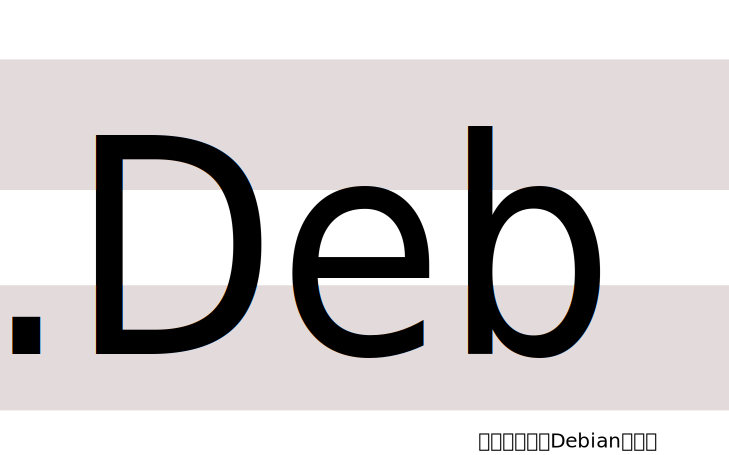
\includegraphics{image-assets/dotdeb.pdf}\\
\hfill{}\debmtgyear{}年\debmtgmonth{}月\debmtgdate{}日

% ここはアップデートすること
% 全角文字にしないとフォントのサイズが合わないので注意
\rotatebox{10}{\fontsize{30}{30} {\gt Etherpad特集}}\\

\vspace*{-2cm}
\hfill{}\includegraphics[height=6cm]{image-assets/openlogo-nd.eps}
\end{titlepage}

\newpage

\begin{minipage}[b]{0.2\hsize}
 \definecolor{titleback}{gray}{0.9}
 \colorbox{titleback}{\rotatebox{90}{\fontsize{80}{80} {\gt デビアン勉強会} }}
\end{minipage}
\begin{minipage}[b]{0.8\hsize}
\hrule
\vspace{2mm}
\hrule
\begin{multicols}{2}
\tableofcontents
\end{multicols}
\vspace{2mm}
\hrule
\end{minipage}

\dancersection{最近のDebian関連のミーティング報告}{杉本 典充}

\subsection{2021年1月度 東京エリア・関西合同Debian勉強会}

2021年1月16日(土)に東京エリアDebian勉強会と関西Debian勉強会の合同で
オンラインによるDebian勉強会を開催しました。参加者は11名でした。

セミナーは上川さんによる「DebianでのNode.js」および参加者全員参加によるBoF「2021年の活動への抱負」を行いました。

セミナー「DebianでのNode.js」ではNode.jsで使われるjavascriptの言語仕様の変遷、バージョン番号の見方の説明がありました。その後DebianでNode.jsを使う方法やDebianパッケージで配布するNode.js関連パッケージのパッケージングルールの説明がありました。ただ、Node.jsの開発が活発に行われているがゆえにDebianの安定版で配布するNode.jsパッケージは古いバージョンになりがちという問題もあるとのことです。そのためNode.jsをDebianで使うには残念ながらNode.jsの本家サイトが配布するパッケージをインストールして使うのが無難ということでした。

BoF「2021年の活動への抱負」 では2021年に何を学習していくとよいかのアイデアを参加者で出し合いました。出てきたアイデアは以下URLの議事録にまとめました。

\url{https://tokyodebian-team.pages.debian.net/2021-01_tokyodebian_bof.txt}

その後、Debianの次期安定版「bullseye」のリリースに向けた進捗の確認、
Debianの最近の動向について情報交換を行いました。

\dancersection{事前課題}{杉本 典充}

今回の事前課題は以下です。

\begin{enumerate}
\item ModSecurityというソフトウェアを知っていましたか。
\item Etherpadというソフトウェアを知っていましたか。
\end{enumerate}

%この課題に対して提出いただいた内容は以下です。

\begin{multicols}{2}
{\small
\begin{prework}{ dictoss }
  \begin{enumerate}
  \item (なし)
  \end{enumerate}
\end{prework}

\begin{prework}{ uwabami }
  \begin{enumerate}
  \item (なし)
  \end{enumerate}
\end{prework}

}
\end{multicols}

%\dancersection{Debian Trivia Quiz}{username}
%
%Debianの昨今の話題についてのQuizです。
%
%今回の出題範囲は\url{debian-devel-announce@lists.debian.org} や \url{debian-news@lists.debian.org}などに投稿された内容からです。
%
%\begin{multicols}{2}
%%; whizzy-master ../debianmeetingresume201211.tex
% $B0J>e$N@_Dj$r$7$F$$$k$?$a!"$3$N%U%!%$%k$G(B M-x whizzytex $B$9$k$H!"(Bwhizzytex$B$,MxMQ$G$-$^$9!#(B
%

\santaku
{DebConf13 $B$N3+:ECO$H3+:EF|$O!)(B}
{$BF|K\!"El5~ET(B 6$B7n(B20$BF|(B}
{$B%K%+%i%0%"(B $B%^%J%0%"(B 7$B7n(B8-14$BF|(B}
{$B%9%$%9!"%t%)!<%^%k%-%e(B 8$B7n(B11-18$BF|(B}
{C}
{$B%K%+%i%0%"$O(BDebConf12$B$N3+:ECO$G$9!#(B
DebConf13$B$O%9%$%9$N%-%c%s%WCO$G3+:E$G$9!#(B
6/20$B$O3'$5$sM=Dj$r6u$1$F$*$-$^$7$g$&!#(B}

\santaku
{$B@$3&$N(BWeb$B%5!<%P$G:G$b?M5$$N$"$k(BLinux $B%G%#%9%H%j%S%e!<%7%g%s(B(W3Techs$BD4$Y(B)$B$O!)(B}
{CentOS}
{Debian}
{Ubuntu}
{B}
{\url{http://w3techs.com/technologies/history_details/os-linux}$B$K7k2L$N%0%i%U$,$"$j$^$9!#(B
$B8=:_(B Linux $B$r;HMQ$7$F$$$k(B web $B%5!<%P$N(B 32.9\% $B$,(B Debian $B$rMxMQ$7$F$*$j!"$=$N3d9g$O8=:_$bA}2C$rB3$1$F$$$k$=$&$G$9!#(B}

\santaku
{Ben Hutchings $B$5$s$,<!4|(B Debian $B0BDjHG$H0l=o$K=P2Y$5$l$k(B Linux $B%+!<%M%k$K(B (3.2 $B7ONs$N(B mainline $B$K$OL5$$(B) $BDI2C5!G=$,Ek:\$5$l$kM=Dj$G$"$k$H=R$Y$F$$$^$9!#(B
$BB?$/$NDI2CE@$NCf$K4^$^$l$J$$$b$N$O2?!)(B}
{PREEMPT\_RT}
{Hyper-V guest drivers$B$N6/2=(B}
{ARM64/AArch64$B%"!<%-%F%/%A%c%5%]!<%H(B}
{C}
{Ben Hutchings $B$5$s$O(BDebian $B%+!<%M%k%A!<%`$N%a%s%P!<$G$"$j!"(Bkernel.org $B$N(B 3.2.y $B0BDjHG7ONs$N%a%s%F%J$G$9!#(BHyper-V guest drivers$B$O(Bmainline kernel$B$G(B3.2$B$K$b4^$^$l$F$$$^$9$,!"$h$j2~A1$5$l$?(B3.4$B$+$i$N=$@5$,F3F~$5$l$^$9!#(B
PREEMPT\_RT$B$O%O!<%I%j%"%k%?%$%`$r<B8=$9$k$?$a$N(BPatch$B!"(B
linux-image-rt-amd64 , linux-image-rt-686-pae $B$N(Bmetapackage$B$G;HMQ$G$-$^$9!#(B
$B?7$7$$(BARM 64$B%S%C%H%"!<%-%F%/%A%c%5%]!<%H$O(Bmainline kernel 3.7$B$+$i(B}

\santaku
{Wookey$B$5$s$,%"%J%&%s%9$7$?(Balpha$BHG$N(BDebian port arm64 image$B$O!)(B}
{Debian/Ubuntu port image}
{Debian/KFreeBSD port image}
{Debian/GnuHurd port image}
{A}
{self-bootstrapp(non x86)$BBP1~$H$N$3$H$G$9!#(B\url{http://wiki.debian.org/Arm64Port}$B$G%9%F!<%?%9$,3NG'$G$-$^$9!#(B}

\santaku
{700,000$BHVL\$N%P%0$,Js9p$5$l$?F|$rEv$F$k(B700000thBugContest$B$N7k2L$,=P$^$7$?!#$=$NM=A[F|$HJs9pF|$O!)(B}
{$BM=A[F|(B:2013/02/04$B!"Js9pF|(B:2013/02/14}
{$BM=A[F|(B:2013/02/07$B!"Js9pF|(B:2013/02/14}
{$BM=A[F|(B:2013/02/14$B!"Js9pF|(B:2013/02/07}
{C}
{$B:G$b6a$$(B2013/02/14$B$rM=A[$7$?(BChristian Perrier$B$5$s$,Ev$F$^$7$?!#7k2L$O(B\url{http://wiki.debian.org/700000thBugContest}$B$G8x3+$5$l$F$$$^$9!#(B
$B$^$?!"(B800,000/1,000,000$BHVL\$N%P%0$,Js9p$5$l$kF|$rEv$F$k%3%s%F%9%H(B\url{http://wiki.debian.org/800000thBugContest}$B$b3+:E$5$l$F$$$^$9!#(B}

\santaku
{master.debian.org$B$,?7$7$$5!3#$K0\9T$5$l$^$7$?!#$3$l$O2?$N%5!<%P$G$7$g$&$+(B $B!)(B}
{@debian.org$B$N%a!<%k%5!<%P(B}
{$B%Q%C%1!<%8$N%^%9%?!<%5!<%P(B}
{$B%Q%C%1!<%8$N%9%]%s%5!<(B(mentor)$B$rC5$9%5!<%P(B}
{A}
{$B8E$$%5!<%P$O%G%#%9%/>c32Ey$,$"$C$?$N$G!"<wL?$HH=CG$5$l!"%G!<%?$,B;<:$9$kA0$K?7$7$$%5!<%P$K0\9T$5$l$^$7$?!#(Bftp-master.debian.org$B$O(BDebian$B$N(B official package $B%j%]%8%H%j$G$9!#%Q%C%1!<%8$N%9%]%s%5!<(B(mentor)$B$rC5$9$N$O(Bmentors.debian.net$B!#(B }

\santaku
{pbuilder$B$K(Bclang support$B$,DI2C$5$l$^$7$?!#C/$,=q$$$?%Q%C%A$G$7$g$&$+!)(B}
{Sylvestre Ledru}
{Junichi Uekawa}
{Hideki Yamane}
{C}
{Debian$B$N(BClang$B%5%]!<%H$OCe!9$H?J$s$G$$$^$9!#(B}

\santaku
{DPN - 2013$BG/(B3$B7n(B4$BF|9f$K<h$j>e$2$i$l$?F|K\$N%$%Y%s%H$O(B}
{Open Source Conference 2013 Tokyo/Spring}
{Open Source Conference 2013 Hamamatu}
{Open Source Conference 2013 Tokushima}
{A}
{\url{http://henrich-on-debian.blogspot.jp/2013/02/open-source-conference-2013-tokyospring.html} $B>\:Y$O8e$[$I!#(B}


%\end{multicols}


% % (query-replace-regexp "<.*?>" "")
% % (query-replace-regexp "^[    ]\+" "")

%-------------------------------------------------------------------------------
\dancersection{Webブラウザでメモの同時共有ができる Etherpad liteの紹介}{杉本典充}
%-------------------------------------------------------------------------------

\subsection{はじめに}

Debian 勉強会を進行をするにあたり、参加者が同時にメモの編集ができる環境がほしいと思っていました。
Web ブラウザを使って複数人が同時にメモの参照や編集ができるツールである「Etherpad lite」を使ってみました。

\subsection{Etherpad と Etherpad lite について}

Etherpad(\url{https://etherpad.org/})とは、Web ブラウザを使って複数人が同時にリアルタイムでメモの参照と編集ができるオープンソースソフトウェア\footnote{\url{https://github.com/ether/etherpad-lite}}です。

歴史的には(初代の) Etherpad は 2008 年に etherpad.com(現在は etherpad.org へリダイレクトされる) でプロプラエタリなサービスとして登場し、Java と Scala で実装したものでした。その後 2009 年に etherpad.com は Google に買収され、買収の直後に etherpad のソースコードが Apache License の元で公開されてオープンソースとなりました\footnote{\url{https://code.google.com/archive/p/etherpad/}}\footnote{リリースアナウンス \url{https://web.archive.org/web/20091221023828/http://etherpad.com/ep/blog/posts/etherpad-open-source-release}}。

(初代の)Etherpad がオープンソースで公開された後、2011年8月22日に JavaScript と Node.js で Etherpad の機能を再実装した「etherpad-lite」の ver 1.0 が登場しました。etherpad の開発を行う The Etherpad Foundation は今後 etherpad-lite の開発に専念することを決めたようで、(初代の)Etherpad は 2013 年に開発を終了しています。なお、etherpad-lite については The Etherpad Foundation の元で現在でも開発が続けられています。

こうした背景があり(初代の)"Etherpad" の開発は既に終了していることから、現在では単に "etherpad" というと「etherpad-lite」を指すようになっています\footnote{\url{https://etherpad.org/\#download} のダウンロード先のリンクは etherpad-lite になっています。}。


\subsection{Etherpad liteにたどり着くまでの利用変遷}

だいぶ前となりますが Web ブラウザを使って複数人が同時にメモを編集でき無料で使える Web サービスとしてtitanpad.com\footnote{ソースコードのアーカイブはこちら \url{https://github.com/titanpad/titanpad}} がありました。titanpad.com は便利なサービスのためDebian勉強会や他の勉強会でも利用されていましたが、2017年12月31日をもってサービスを終了しました\footnote{\url{http://blog.titanpad.com/2016/11/shutting-down-titanpad_12.html}}。

その後、Debian 勉強会ではメモの同時編集ツールとして DebConf などでも使われている gobby \footnote{\url{https://github.com/gobby/gobby/wiki}} を使っていましたが gobby は使いにくいという声(特にdebianを使っていない方)もあり、Web ブラウザで利用できるメモの同時編集ツールを再度探していました。

ツールを探していく中で Web サービスはでなく自分のサーバにインストールするタイプの「etherpad-lite」があることを知り、最近は Debian 勉強会に導入し BoF で利用しています。

\subsection{Etherpad liteのインストール}

\subsubsection{Node.js のインストール}

etherpad-lite のインストール手順は以下URLに記載されています。

\url{https://github.com/ether/etherpad-lite#installation}

現在のetherpad-lite-1.8.8 では nodejs-10.17.0 以上の環境が必要であり、以下コマンドでnodejsをインストールします。

\begin{commandline}
$ curl -sL https://deb.nodesource.com/setup_14.x | sudo -E bash -
# apt install -y nodejs
\end{commandline}

\subsubsection{Etherpad liteのダウンロードと配置}

etherpad-lite のプログラムを以下URLからダウンロードして、/optに配置します。

\begin{commandline}
# wget https://github.com/ether/etherpad-lite/archive/1.8.8.zip
# cp 1.8.8.zip /opt/etherpad-lite-1.8.8.zip
# cd /opt
# unzip etherpad-lite-1.8.8.zip
# ln -s etherpad-lite-1.8.8 etherpad-lite  
\end{commandline}

etherpad-lite のプログラムを実行するスクリプト "bin/run.sh" は、実行時にプログラムを置いているディレクトリの配下に "node\_modules" ディレクトリを作成して依存ライブラリを自動でダウンロードします。そのため、プログラムを実行するユーザはこのディレクトリに書き込み権限を持つ必要があります。プログラムを実行するユーザとグループとして "etherpad" ユーザ及びグループを作成し、etherpad-liteディレクトリとファイルのオーナーとグループを変更します。

\begin{commandline}
# adduser etherpad
# chown -fR etherpad:etherpad /opt/etherpad-lite-1.8.8
# ls -l /opt/etherpad-lite-1.8.8
合計 180
-rw-r--r-- 1 etherpad etherpad    64  2月 18 22:17 APIKEY.txt
-rw-r--r-- 1 etherpad etherpad 40276  2月 16 02:47 CHANGELOG.md
-rw-r--r-- 1 etherpad etherpad  8217  2月 16 02:47 CONTRIBUTING.md
-rw-r--r-- 1 etherpad etherpad  1681  2月 16 02:47 Dockerfile
-rw-r--r-- 1 etherpad etherpad 11353  2月 16 02:47 LICENSE
-rw-r--r-- 1 etherpad etherpad   849  2月 16 02:47 Makefile
-rw-r--r-- 1 etherpad etherpad  8229  2月 16 02:47 README.md
-rw-r--r-- 1 etherpad etherpad   118  2月 16 02:47 SECURITY.md
-rw-r--r-- 1 etherpad etherpad    64  2月 18 22:16 SESSIONKEY.txt
lrwxrwxrwx 1 etherpad etherpad     7  2月 18 22:10 bin -> src/bin
drwxr-xr-x 6 etherpad etherpad  4096  2月 16 02:47 doc
drwxr-xr-x 2 etherpad etherpad  4096  2月 16 02:47 node_modules
-rw-r--r-- 1 etherpad etherpad 21152  2月 16 02:47 settings.json.docker
-rw-r--r-- 1 etherpad etherpad 19209  2月 16 02:47 settings.json.template
drwxr-xr-x 9 etherpad etherpad  4096  2月 18 22:17 src
-rw-r--r-- 1 etherpad etherpad    51  2月 16 02:47 start.bat
lrwxrwxrwx 1 etherpad etherpad     9  2月 18 22:10 tests -> src/tests
drwxr-xr-x 2 etherpad etherpad  4096  2月 18 22:34 var
\end{commandline}

次に設定ファイル "settings.json" を配置します。設定内容はひとまずデフォルトのコピーとしておきます。

\begin{commandline}
# cd /opt/etherpad-lite-1.8.8
# cp -p settings.json.template settings.json
\end{commandline}

etherpad-lite を起動できることを確認してみます。

\begin{commandline}
# cd /opt/etherpad-lite-1.8.8
# sudo -u etherpad bin/run.sh
\end{commandline}

以下のURLのアクセスすると etherpad-lite に接続できます。

\url{http://localhost:9001/p/debianmeeting20210220}


\subsubsection{systemctlで起動できるようserviceファイルを配置する}

毎回手動で etherpad-lite を起動するのも面倒です。そのため、systemctl から起動できるように設定します。

systemctl で起動できるように以下のような service ファイルを作成します。

\begin{commandline}
# vi /etc/systemd/system/etherpad-lite.service

[Unit]
Description=etherpad-lite

[Service]
Type=simple
ExecStart=/opt/etherpad-lite/bin/run.sh
WorkingDirectory=/opt/etherpad-lite
Restart=always
RestartSec=10
User=etherpad
Group=etherpad
Environment=NODE_ENV=production

[Install]
WantedBy=multi-user.target
\end{commandline}

systemctl daemon-reload を実行して追加した service ファイルを systemd に再読み込みさせ、etherpad-lite を起動します。

\begin{commandline}
# systemctl daemon-reload
# systemctl start etherpad-lite
# systemctl status etherpad-lite
● etherpad-lite.service - etherpad-lite
   Loaded: loaded (/etc/systemd/system/etherpad-lite.service; disabled; vendor p
   Active: active (running) since Fri 2021-02-19 22:11:05 JST; 4s ago
 Main PID: 26451 (run.sh)
    Tasks: 13 (limit: 1149)
   Memory: 155.0M
   CGroup: /system.slice/etherpad-lite.service
           ├─26451 /bin/sh /opt/etherpad-lite/bin/run.sh
           ├─26454 /bin/sh src/bin/installDeps.sh
           └─26491 npm
\end{commandline}

これで、systemctl で管理しつつ etherpad-lite を起動できるようになりました。


\subsubsection{WebサーバへのアクセスをEtherpad liteへリバースプロキシする}

これまでの手順で起動できるようになった etherpad-lite の状態では、9001 番ポートで待ち受けします。クライアントとなる Web ブラウザから etherpad-lite サーバの 9001 番ポートへ接続する場合に、利用するネットワークやファイアウォール設定などの環境によって接続できない場合があります。

以下URLを参考に apache2.4 の mod\_proxy を使ってリバースプロキシの設定を行い、クライアントからは80番ポート(http://)、または 443 番ポート(https://)で接続できるようにしてみました。

\url{https://github.com/ether/etherpad-lite/wiki/How-to-put-Etherpad-Lite-behind-a-reverse-Proxy}

まずは apache2.4 をインストールします。

\begin{commandline}
# apt update
# apt install apache2
\end{commandline}  

apache2.4 の mod\_proxy などの利用するモジュールを有効にします。

\begin{commandline}
# a2enmod proxy
# a2enmod proxy_http
# a2enmod proxy_balancer
# a2enmod lbmethod_byrequests
# a2enmod rewrite
# a2enmod proxy_wstunnel
\end{commandline}

etherpad-lite の 9001 番ポートへリバースプロキシする設定ファイル "etherpad-lite.conf" を作成します。

\begin{commandline}
# vi /etc/apache2/conf-available/etherpad-lite.conf

    ProxyVia On
    ProxyRequests Off
    ProxyPreserveHost on

    <Location /etherpad/>
        ProxyPass http://localhost:9001/ retry=0 timeout=30
        ProxyPassReverse http://localhost:9001/
    </Location>
    <Location /etherpad/socket.io>
        # This is needed to handle the websocket transport through the proxy, since
        # etherpad does not use a specific sub-folder, such as /ws/ to handle this kind of traffic.
        # Taken from https://github.com/ether/etherpad-lite/issues/2318#issuecomment-63548542
        # Thanks to beaugunderson for the semantics
        RewriteEngine On
        RewriteCond %{QUERY_STRING} transport=websocket    [NC]
        RewriteRule /(.*) ws://localhost:9001/socket.io/$1 [P,L]
        ProxyPass http://localhost:9001/socket.io retry=0 timeout=30
        ProxyPassReverse http://localhost:9001/socket.io
    </Location>

    <Proxy *>
      Options FollowSymLinks MultiViews
      AllowOverride All
      Order allow,deny
      allow from all
    </Proxy>
\end{commandline}

a2enconf コマンドを実行して "etherpad-lite.conf" の設定を apache2.4 へ組み込み、apache2.4 を reload します。

\begin{commandline}
# a2enconf etherpad-lite
Enabling conf etherpad-lite.
To activate the new configuration, you need to run:
  systemctl reload apache2

# systemctl reload apache2
\end{commandline}

これで以下の URL のように クライアントから etherpad-lite サーバへ 80 番ポートに接続して使えるようになりました。

\url{http://www.pcdennokan.wjg.jp/etherpad/p/debianmeeting20210220}


\subsubsection{etherpad-lite の設定}

デフォルトの設定ファイル "settings.json" はクライアントからのアクセスに認証を必要としない設定になっています。最低限の認証を行えるように設定する例を紹介します。以下の設定は1つのアカウントを全ユーザで共用する設定になっています。

\begin{commandline}
--- settings.json.template      2021-02-16 02:47:33.000000000 +0900
+++ settings.json       2021-02-18 22:15:43.144967658 +0900
@@ -315,7 +315,7 @@
    *
    * Note: "/admin" always requires authentication.
    */
-  "requireAuthentication": false,
+  "requireAuthentication": true,

   /*
    * Require authorization by a module, or a user with is_admin set, see below.
@@ -428,22 +428,26 @@
    *          follow the section "secure your installation" in README.md
    */

-  /*
   "users": {
     "admin": {
       // 1) "password" can be replaced with "hash" if you install ep_hash_auth
       // 2) please note that if password is null, the user will not be created
-      "password": "changeme1",
+      "password": "adminpassword",
       "is_admin": true
     },
-    "user": {
+    //"user": {
       // 1) "password" can be replaced with "hash" if you install ep_hash_auth
       // 2) please note that if password is null, the user will not be created
-      "password": "changeme1",
+    //  "password": "changeme1",
+    //  "is_admin": false
+    //}
+    "myuser": {
+       // 1) "password" can be replaced with "hash" if you install ep_hash_auth
+       // 2) please note that if password is null, the user will not be created
+      "password": "myuserpassword",
       "is_admin": false
     }
   },
-  */
\end{commandline}

そのほか、\url{https://static.etherpad.org/index.html} で多数のetherpad-lite 用のプラグインがありますので実用するにあたり自分の利用方法にあるものを探してみるとよいと思います。

\subsection{おわりに}

etherpad-lite の歴史とインストール手順を説明し、etherpad-lite サーバを作ってみました。
最近はクラウドサービスの Office 系アプリケーションでも同時編集が可能になっているサービスもありますが、オープンソースなアプリケーションを使って複数人でメモの同時編集する環境を構築できますのでオープンソースライフを楽しみつつ実用していただけるのでないかと思います。


\subsection{参考情報}

\begin{itemize}
\item etherpad.com \\ \url{https://etherpad.org/}
\item EtherPad Open Source Release \\ \url{https://web.archive.org/web/20091221023828/http://etherpad.com/ep/blog/posts/etherpad-open-source-release}
\item How to put Etherpad Lite behind a reverse Proxy \\ \url{https://github.com/ether/etherpad-lite/wiki/How-to-put-Etherpad-Lite-behind-a-reverse-Proxy}
\end{itemize}


% 冊子にするために、4の倍数にする必要がある。
% そのための調整
\dancersection{メモ}{}
\mbox{}\newpage
\mbox{}\newpage

\vspace*{15cm}
\hrule
\vspace{2mm}
\includegraphics[width=2cm]{image-assets/openlogo-nd.eps}
\noindent \Large \bf Debian 勉強会資料\\
\noindent \normalfont \debmtgyear{}年\debmtgmonth{}月\debmtgdate{}日 \hspace{5mm}  初版第1刷発行\\
\noindent \normalfont 東京エリア Debian 勉強会 (編集・印刷・発行)\\
\hrule
\end{document}
